\section{System description}
\label{sec:system}

Probe runs eight stages in sequence. Stages 1 and 2 are single-call; stages 3 through 7 fan out across three branches running in parallel via \texttt{Promise.all} and real git worktrees; stage 8 synthesizes the single surviving branch (Figure \ref{fig:pipeline}). Every stage reads inputs from files on disk and writes outputs to files on disk; no conversation context is shared across stages. Every output that crosses a stage boundary validates against a JSON schema; failure triggers a repair pass, and a second failure throws.

\begin{figure}[ht]
\centering
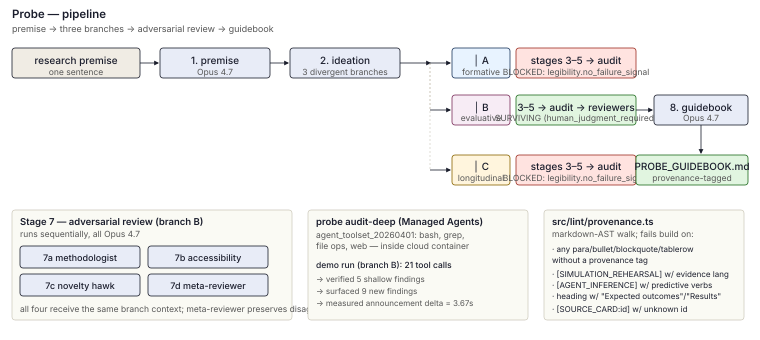
\includegraphics[width=\textwidth]{figures/pipeline.svg}
\caption{The Probe pipeline on the demo run. Stage 1 interrogates the premise; stage 2 produces three divergent branches; stages 3--7 run per-branch in parallel; stage 8 assembles a guidebook from the surviving branch. Branches A and C were blocked by the capture-risk audit on \texttt{legibility.no\_failure\_signal}; branch B survived to adversarial review and guidebook assembly with meta-reviewer verdict \texttt{human\_judgment\_required}. The two lower panels show the reviewer panel (four Opus 4.7 sessions; meta-reviewer preserves disagreement) and the \texttt{probe audit-deep} Managed Agents extension (21 tool calls on the demo run; measured a 3.67-second announcement-duration delta). The right panel names the specific failure modes the markdown-AST provenance linter rejects.}
\label{fig:pipeline}
\end{figure}

\subsection{Model routing}

The routing rule is: Opus 4.7 for stages that require skeptical judgment, evidence-span selection, sustained role-separated stance, or long-context synthesis under provenance constraints; Sonnet 4.6 for retrieval over a small curated corpus and for schema-enforced templating. Table~\ref{tab:routing} lists the stages and the reason each is routed where it is.

\begin{table}[ht]
\centering
\small
\caption{Model routing by stage. Per-run cost figures are the median across three benchmark runs.}
\label{tab:routing}
\begin{tabular}{@{}llll@{}}
\toprule
\# & Stage & Model & Reason \\
\midrule
1 & Premise interrogation & Opus 4.7 & Skeptical PI voice, flattery resistance \\
2 & Solution ideation & Opus 4.7 & Divergence constraints across four axes \\
3 & Literature grounding & Sonnet 4.6 & Corpus retrieval with a fixed allow-list \\
4 & Prototype specification & Sonnet 4.6 & Structured templating with schema enums \\
5 & Simulated walkthrough & Opus 4.7 & Hedged rehearsal voice, discipline on ``evidence'' \\
6 & Capture-risk audit & Opus 4.7 & Normative reasoning, evidence-span selection \\
7 & Adversarial review (×3 + meta) & Opus 4.7 & Sustained role-separation, refuse consensus \\
8 & Guidebook assembly & Opus 4.7 & Long-context synthesis, provenance discipline \\
\bottomrule
\end{tabular}
\end{table}

\subsection{Capture-risk audit}

The capture-risk auditor is the project's load-bearing normative step. It fires sixteen patterns across four axes: Capacity, Agency, Exit, and Legibility. The axes come from Buijsman, Carter, and Bermúdez's framing of domain-specific autonomy \citep{buijsman2025autonomy} and from Illich's distinction between convivial and industrial tools \citep{illich1973conviviality}. Each pattern has a trigger heuristic, an evidence template, and a default score on the scale $\{-2, -1, 0, +1, +2\}$: minus-two is ``capture,'' minus-one is ``drift,'' zero is ``neutral,'' plus-one is ``scaffold,'' plus-two is ``cultivate.''

The verdict rule is strict: any minus-two finding produces \texttt{BLOCKED}; two or more minus-ones produce \texttt{REVISION\_REQUIRED}; otherwise \texttt{PASSED}. The orchestrator computes the verdict from the findings, overwriting any inconsistent self-report by the model. Without this override the auditor's own arithmetic drifted in roughly one in three development trials. The model does pattern judgment and evidence-span selection; the orchestrator handles the sum.

A minus-two finding triggers a \texttt{WORKSHOP\_NOT\_RECOMMENDED.md} report that names the fired pattern, quotes the evidence span, lists the findings that together carried the verdict, and suggests what specific revision would unblock the branch. The report ends with a \texttt{[HUMAN\_REQUIRED]} block asking the researcher to confirm the pattern fired correctly rather than flagged a manipulation-under-test as paternalism. Figure \ref{fig:audit_finding} shows the exact shape of a fired finding: pattern id, axis, score, a quoted evidence span from the prototype spec, the auditor's rationale, and the resulting branch verdict. The evidence span is the structural feature that distinguishes the audit from general-purpose critique --- a quoted passage the researcher can open and verify, not a free-form objection.

\begin{figure}[ht]
\centering
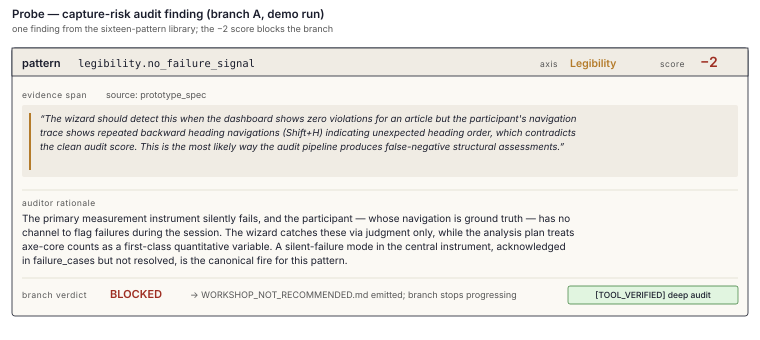
\includegraphics[width=\textwidth]{figures/audit_finding.svg}
\caption{A fired capture-risk pattern from branch A of the demo run. The pattern \texttt{legibility.no\_failure\_signal} scores the branch at $-2$, which the verdict rule escalates to \texttt{BLOCKED}. The evidence span is a verbatim quote from the prototype spec --- the auditor must ground the finding in a passage the researcher can open, rather than in a rephrased summary. The same evidence span is what the \texttt{[TOOL\_VERIFIED]} deep-audit then measures quantitatively in the \texttt{probe audit-deep} extension.}
\label{fig:audit_finding}
\end{figure}

\subsection{Adversarial review panel}

Stage 7 runs three reviewer agents in sequence against the same branch context. Each agent operates under a system prompt that forbids preamble, requires a first-line ``decisive weakness,'' and lists specific generic critiques that are banned unless attached to a quoted evidence span.

The methodologist audits validity, confounds, recruitment adequacy, IRB framing, and the match between claim and method. The accessibility advocate applies the Kafer political-relational model of disability \citep{kafer2013feminist}, catching paternalistic defaults, extractive recruitment framings, and curative imaginary language. The novelty hawk cross-references the source-card corpus and identifies adjacent literature the proposal does not cite; it may name papers outside the corpus, but only inside a dedicated \texttt{uncited\_adjacent\_literature} output field that the guidebook assembler renders as \texttt{[UNCITED\_ADJACENT]} elements the researcher must verify before grounding.

The meta-reviewer reads the three reviewer findings and produces a disagreement matrix classified as one of: \texttt{consensus}, \texttt{legitimate\_methodological\_split}, \texttt{legitimate\_normative\_split}, \texttt{spurious\_surface\_disagreement}, or \texttt{single\_reviewer\_outlier}. The meta-reviewer is explicitly forbidden from classifying a legitimate split as consensus. Its final verdict is one of \texttt{accept\_revise}, \texttt{reject}, or \texttt{human\_judgment\_required}. The last of these is not a failure state; it is an honest outcome when the three reviewers identify substantive, non-reducible objections.

\subsection{Provenance discipline}

Every paragraph, bullet, blockquote, list item, and table row in a generated guidebook ends with exactly one provenance tag. Eight tags are valid: \texttt{RESEARCHER\_INPUT}, \texttt{SOURCE\_CARD:<id>}, \texttt{SIMULATION\_REHEARSAL}, \texttt{AGENT\_INFERENCE}, \texttt{UNCITED\_ADJACENT}, \texttt{HUMAN\_REQUIRED}, \texttt{DO\_NOT\_CLAIM}, and \texttt{TOOL\_VERIFIED} (the last used only by the Managed Agents deep-audit command).

The linter walks the markdown AST via remark \citep{remark}. It requires a tag on every content-bearing node; rejects any \texttt{[SIMULATION\_REHEARSAL]} element that uses evidence language from a fixed list (``users preferred,'' ``participants found,'' ``findings show,'' ``significant,'' ``validated,'' ``proved,'' ``demonstrated that,'' ``evidence suggests,'' ``data indicates''); rejects any \texttt{[SOURCE\_CARD:id]} that references an id not present in \texttt{corpus/source\_cards/}; rejects any \texttt{[AGENT\_INFERENCE]} element containing predictive-outcome claims (``condition X produces higher Y''); rejects headings containing evidence language or anti-pattern titles like ``Expected outcomes,'' ``Results,'' or ``Findings'' even if the paragraphs below are correctly tagged; and requires at least one \texttt{[HUMAN\_REQUIRED]} element per document. The document-level check is the last of these: a guidebook without a human handoff fails the lint and does not leave the run directory.

\subsection{Managed Agents deep audit}

The shallow capture-risk audit in Stage 6 is a single Messages-API call. It reasons over the prototype spec and the simulated walkthrough, fires the sixteen patterns, and produces evidence spans. It cannot run computations.

The \texttt{probe audit-deep} command spawns a Claude Managed Agent (Opus 4.7 with the \texttt{agent\_toolset\_20260401} that exposes bash, file operations, web search, and grep) inside a managed cloud container with the branch artifacts loaded as files. The agent's task is to take the shallow audit's findings and measure them rather than reason about them.

On branch B of the demo run, the managed agent ran twenty-one tool calls in one session. It computed the announcement-duration delta the shallow audit had described qualitatively (``substantially longer''): the AI-disclosure string is ninety-six characters, sixteen words, about 5.3 seconds of speech at 180 words per minute; the human-framed string is twenty-nine characters, five words, about 1.7 seconds; the delta is 3.67 seconds. It grepped the prototype spec for mechanisms the shallow audit was uncertain about: zero matches for ``byline,'' ``model card,'' ``source link,'' ``editorial policy,'' ``inspect,'' or ``tell me more,'' which confirms two separate Legibility findings with a measured zero. It ran a Friedman-test minimum-detectable-effect-size calculation at $n=8, k=3, \alpha=0.05$ and produced Kendall's $W = 0.374$, which is between medium and large. It checked whether the axe-core WCAG gate the study proposes covers the debrief card and the credibility form; it did not. The agent's final summary reported five shallow-audit findings verified with measurements, zero challenged, and nine new findings the shallow audit had missed.

This is the specific value-add of Managed Agents over direct API calls: the agent measured claims that a single-prompt audit could only paraphrase.
